\documentclass[conference]{IEEEtran}
\IEEEoverridecommandlockouts
% The preceding line is only needed to identify funding in the first footnote. If that is unneeded, please comment it out.
\usepackage{cite}
\usepackage{amsmath,amssymb,amsfonts}
\usepackage{algorithmic}
\usepackage{graphicx}
\usepackage{textcomp}
\usepackage{xcolor}
\def\BibTeX{{\rm B\kern-.05em{\sc i\kern-.025em b}\kern-.08em
    T\kern-.1667em\lower.7ex\hbox{E}\kern-.125emX}}
\begin{document}

\title{Effects of Noise on multi-objective optimiser performance}

\author{\IEEEauthorblockN{BART Number 208912}
\IEEEauthorblockA{\textit{Dept. of Computer Science} \\
\textit{University of Exeter}\\
England, United Kingdom
}
}

\maketitle

\begin{abstract}
This document is a model and instructions for \LaTeX.
This and the IEEEtran.cls file define the components of your paper [title, text, heads, etc.]. *CRITICAL: Do Not Use Symbols, Special Characters, Footnotes, 
or Math in Paper Title or Abstract.
\end{abstract}

\begin{IEEEkeywords}
Multi-objective Evolutionary Algorithm, Noise, Rolling Tide Evolutionary Algorithm, Inverse Generational Distance, Hypervolume measure
\end{IEEEkeywords}

\section{Introduction}
Evolutionary Algorithms (EAs), particularly, genetic algorithms (GA), are known to be robust in the presence of noise \cite{bui2005}. Multi-objective Evolutionary Algorithms (MOEAs) obtain a Pareto set of non-dominated solutions, offering decision-makers more options from which to choose the best solution according to some preference information. MOEAs can be broadly classified into two categories - elitism and non-elitism. With the elitism approach, EMOs employ an external set to store the best solutions in each generation. This set will then be a part of next generation. With this method, the best individuals in each generation are always preserved, and this helps the algorithm to get as close as possible to the Pareto front. In contrast, the non elitism approach has no concept of elitism when it selects individuals for reproduction. In this study, we consider algorithms with an elitism approach \cite{bui2005}. A factor of interest in this study is the existence of noise in optimisation problems, which is inevitable are prevalent in sources such as sensors, actuators, or because of the stochasticity pertaining in some problems such as multi-agent simulations \cite{bui2005}.

\section{Background}
\subsection{MOEAs}
\subsubsection{NSGA-II}
\subsubsection{SPEA2}
\subsubsection{RTEA}
\subsection{Noise}
In a real-world black-box problem, noise takes various forms and can be stochastic in nature. In such cases, the effect of noise could lead to misleading non-dominating solutions which might actually be dominated for a true noiseless problem. \\
In modelling noise as a factor, various researchers have adopted different approaches. Bui \textit{et al.} \cite{bui2005} use an additive factor which are randomly added or subtracted from the real fitness value, such that $F_{noise} = F + noise$, where $F_{noise}$ is fitness function with presence of noise and $F$ is the true fitness function. Fieldsend \textit{et al.} \cite{fieldsend2015} consider a gaussian function of noise to be added with $\mathcal{N} \sim (0, \sigma^{2})$, i.e., a zero-mean isotropic Gaussian noise with standard deviation ($\sigma$) of a constant real number. They consider multiple standard deviation inputs of \{0.00, 0.01, 0.10, 1.00\}, where $\sigma = 0.00$ is the true, noiseless fitness function.
\subsection{Performance metrics}


\section{Research methodology}
\subsection{Problem}

\subsection{Algorithms}
The three MOEAs selected in this study are NSGA-II, SPEA2, and RTEA.
\subsection{Noise magnitude}
The noise magnitude considered in this study is a zero-mean isotropic gaussian noise with standard deviation magnitudes of $\sigma = \{0.00, 0.01, 0.05, 0.1, 1.00\}$, with reference to papers written by Bui \textit{et al.} \cite{bui2005} and Fieldsend \textit{et al.} \cite{fieldsend2015}. This is because the additive nature of noise as described in the former paper has a similar effect to the true pareto front as by gaussian approach of the latter paper.
\begin{figure}[h]
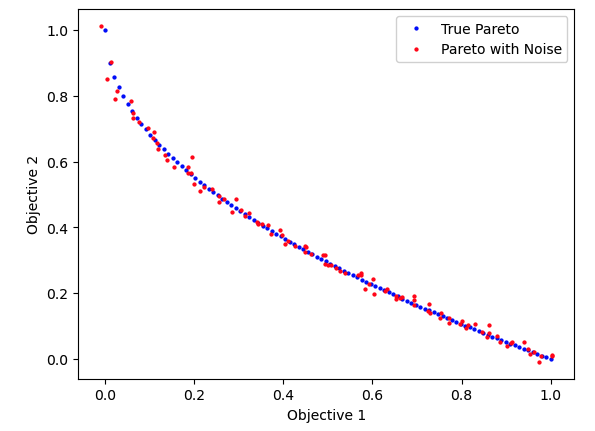
\includegraphics[width=0.5\textwidth]{noise_effect}
\caption{Example of effect of gaussian noise of magnitude $\sigma = 0.01$ on true Pareto front}
\centering
\end{figure}

\subsection{Performance metrics}

\section{Results}

\section{Conclusion}

\section*{Acknowledgment}

The preferred spelling of the word ``acknowledgment'' in America is without 
an ``e'' after the ``g''. Avoid the stilted expression ``one of us (R. B. 
G.) thanks $\ldots$''. Instead, try ``R. B. G. thanks$\ldots$''. Put sponsor 
acknowledgments in the unnumbered footnote on the first page.

\section*{References}

Please number citations consecutively within brackets \cite{b1}. The 
sentence punctuation follows the bracket \cite{b2}. Refer simply to the reference 
number, as in \cite{b3}---do not use ``Ref. \cite{b3}'' or ``reference \cite{b3}'' except at 
the beginning of a sentence: ``Reference \cite{b3} was the first $\ldots$''

Number footnotes separately in superscripts. Place the actual footnote at 
the bottom of the column in which it was cited. Do not put footnotes in the 
abstract or reference list. Use letters for table footnotes.

Unless there are six authors or more give all authors' names; do not use 
``et al.''. Papers that have not been published, even if they have been 
submitted for publication, should be cited as ``unpublished'' \cite{b4}. Papers 
that have been accepted for publication should be cited as ``in press'' \cite{b5}. 
Capitalize only the first word in a paper title, except for proper nouns and 
element symbols.

For papers published in translation journals, please give the English 
citation first, followed by the original foreign-language citation \cite{b6}.

\begin{thebibliography}{00}
\bibitem{b1} G. Eason, B. Noble, and I. N. Sneddon, ``On certain integrals of Lipschitz-Hankel type involving products of Bessel functions,'' Phil. Trans. Roy. Soc. London, vol. A247, pp. 529--551, April 1955.
\bibitem{b2} J. Clerk Maxwell, A Treatise on Electricity and Magnetism, 3rd ed., vol. 2. Oxford: Clarendon, 1892, pp.68--73.
\bibitem{b3} I. S. Jacobs and C. P. Bean, ``Fine particles, thin films and exchange anisotropy,'' in Magnetism, vol. III, G. T. Rado and H. Suhl, Eds. New York: Academic, 1963, pp. 271--350.
\bibitem{b4} K. Elissa, ``Title of paper if known,'' unpublished.
\bibitem{b5} R. Nicole, ``Title of paper with only first word capitalized,'' J. Name Stand. Abbrev., in press.
\bibitem{b6} Y. Yorozu, M. Hirano, K. Oka, and Y. Tagawa, ``Electron spectroscopy studies on magneto-optical media and plastic substrate interface,'' IEEE Transl. J. Magn. Japan, vol. 2, pp. 740--741, August 1987 [Digests 9th Annual Conf. Magnetics Japan, p. 301, 1982].
\bibitem{b7} M. Young, The Technical Writer's Handbook. Mill Valley, CA: University Science, 1989.
\end{thebibliography}
\vspace{12pt}
\color{red}
IEEE conference templates contain guidance text for composing and formatting conference papers. Please ensure that all template text is removed from your conference paper prior to submission to the conference. Failure to remove the template text from your paper may result in your paper not being published.

\end{document}
